
\section{Introduction}
 \textit{Code Obfuscation} seeks to protect valuable assets contained in software from those who have full access to it by making the software difficult to analyze. An obfuscator $\mathcal{O}$ applies a sequence of \textit{code transformations} $\mathcal{T}_1 \circ \mathcal{ T}_2 \circ \mathcal{ T}_3 \circ\ldots$ to an input program $P$ containing an asset $a$, transforming it into a program $P'=\mathcal{O}(P)$, such that $P$ and $P'$ are semantically identical, but extracting $a$ from $P'$ is more difficult than extracting $a$ from $P$. Common assets include cryptographic keys, proprietary algorithms, security checks, etc. Obfuscating transformations are also used to induce {\em diversity}: given an original program $P$, a diversifying obfuscator generates a large number of semantically identical but syntactically different programs $\{P'_1, P'_2,\ldots\}$. Diversity is a defense against {\em class attacks}, where a single attack can successfully target all programs protected with a particular technique.

Attacks on obfuscation (known as \textit{reverse engineering} or \textit{deobfuscation}) aim to defeat the obfuscating transformations by extracting a close facsimile of the asset $a$ from $P'$.

Much work has gone into developing methods to evaluate obfuscating transformations. Fundamental questions we may want to ask include (a) ``how long will asset $a$ survive in the field in a program $P'$ that has been protected with obfuscating transform $\mathcal{T}$?''; (b) ``how do transformations $\mathcal{T}_1$ and $\mathcal{T}_2$ compare with respect to their protective power and performance degradation?''; and (c) ``what level of diversity can transformation $\mathcal{T}$ induce?'' 

Unfortunately, the validity of any theoretical models we develop to answer such questions will ultimately depend on how we define {\em the power of the adversary}.

%While a few empirical evaluations of the behavior of reverse engineers exist, they all suffer from several fundamental problems: (a) small sample sizes, (b) subjects who have limited prior experience with reverse engineering (such as computer science undergraduate students), or (c) subjects who are bound by confidentiality agreements (such as members of professional red teams) resulting in data sets that cannot be published; all of these factors reduce generalizability to real-life adversaries.

%\begin{figure*}[t]
%%\centering
%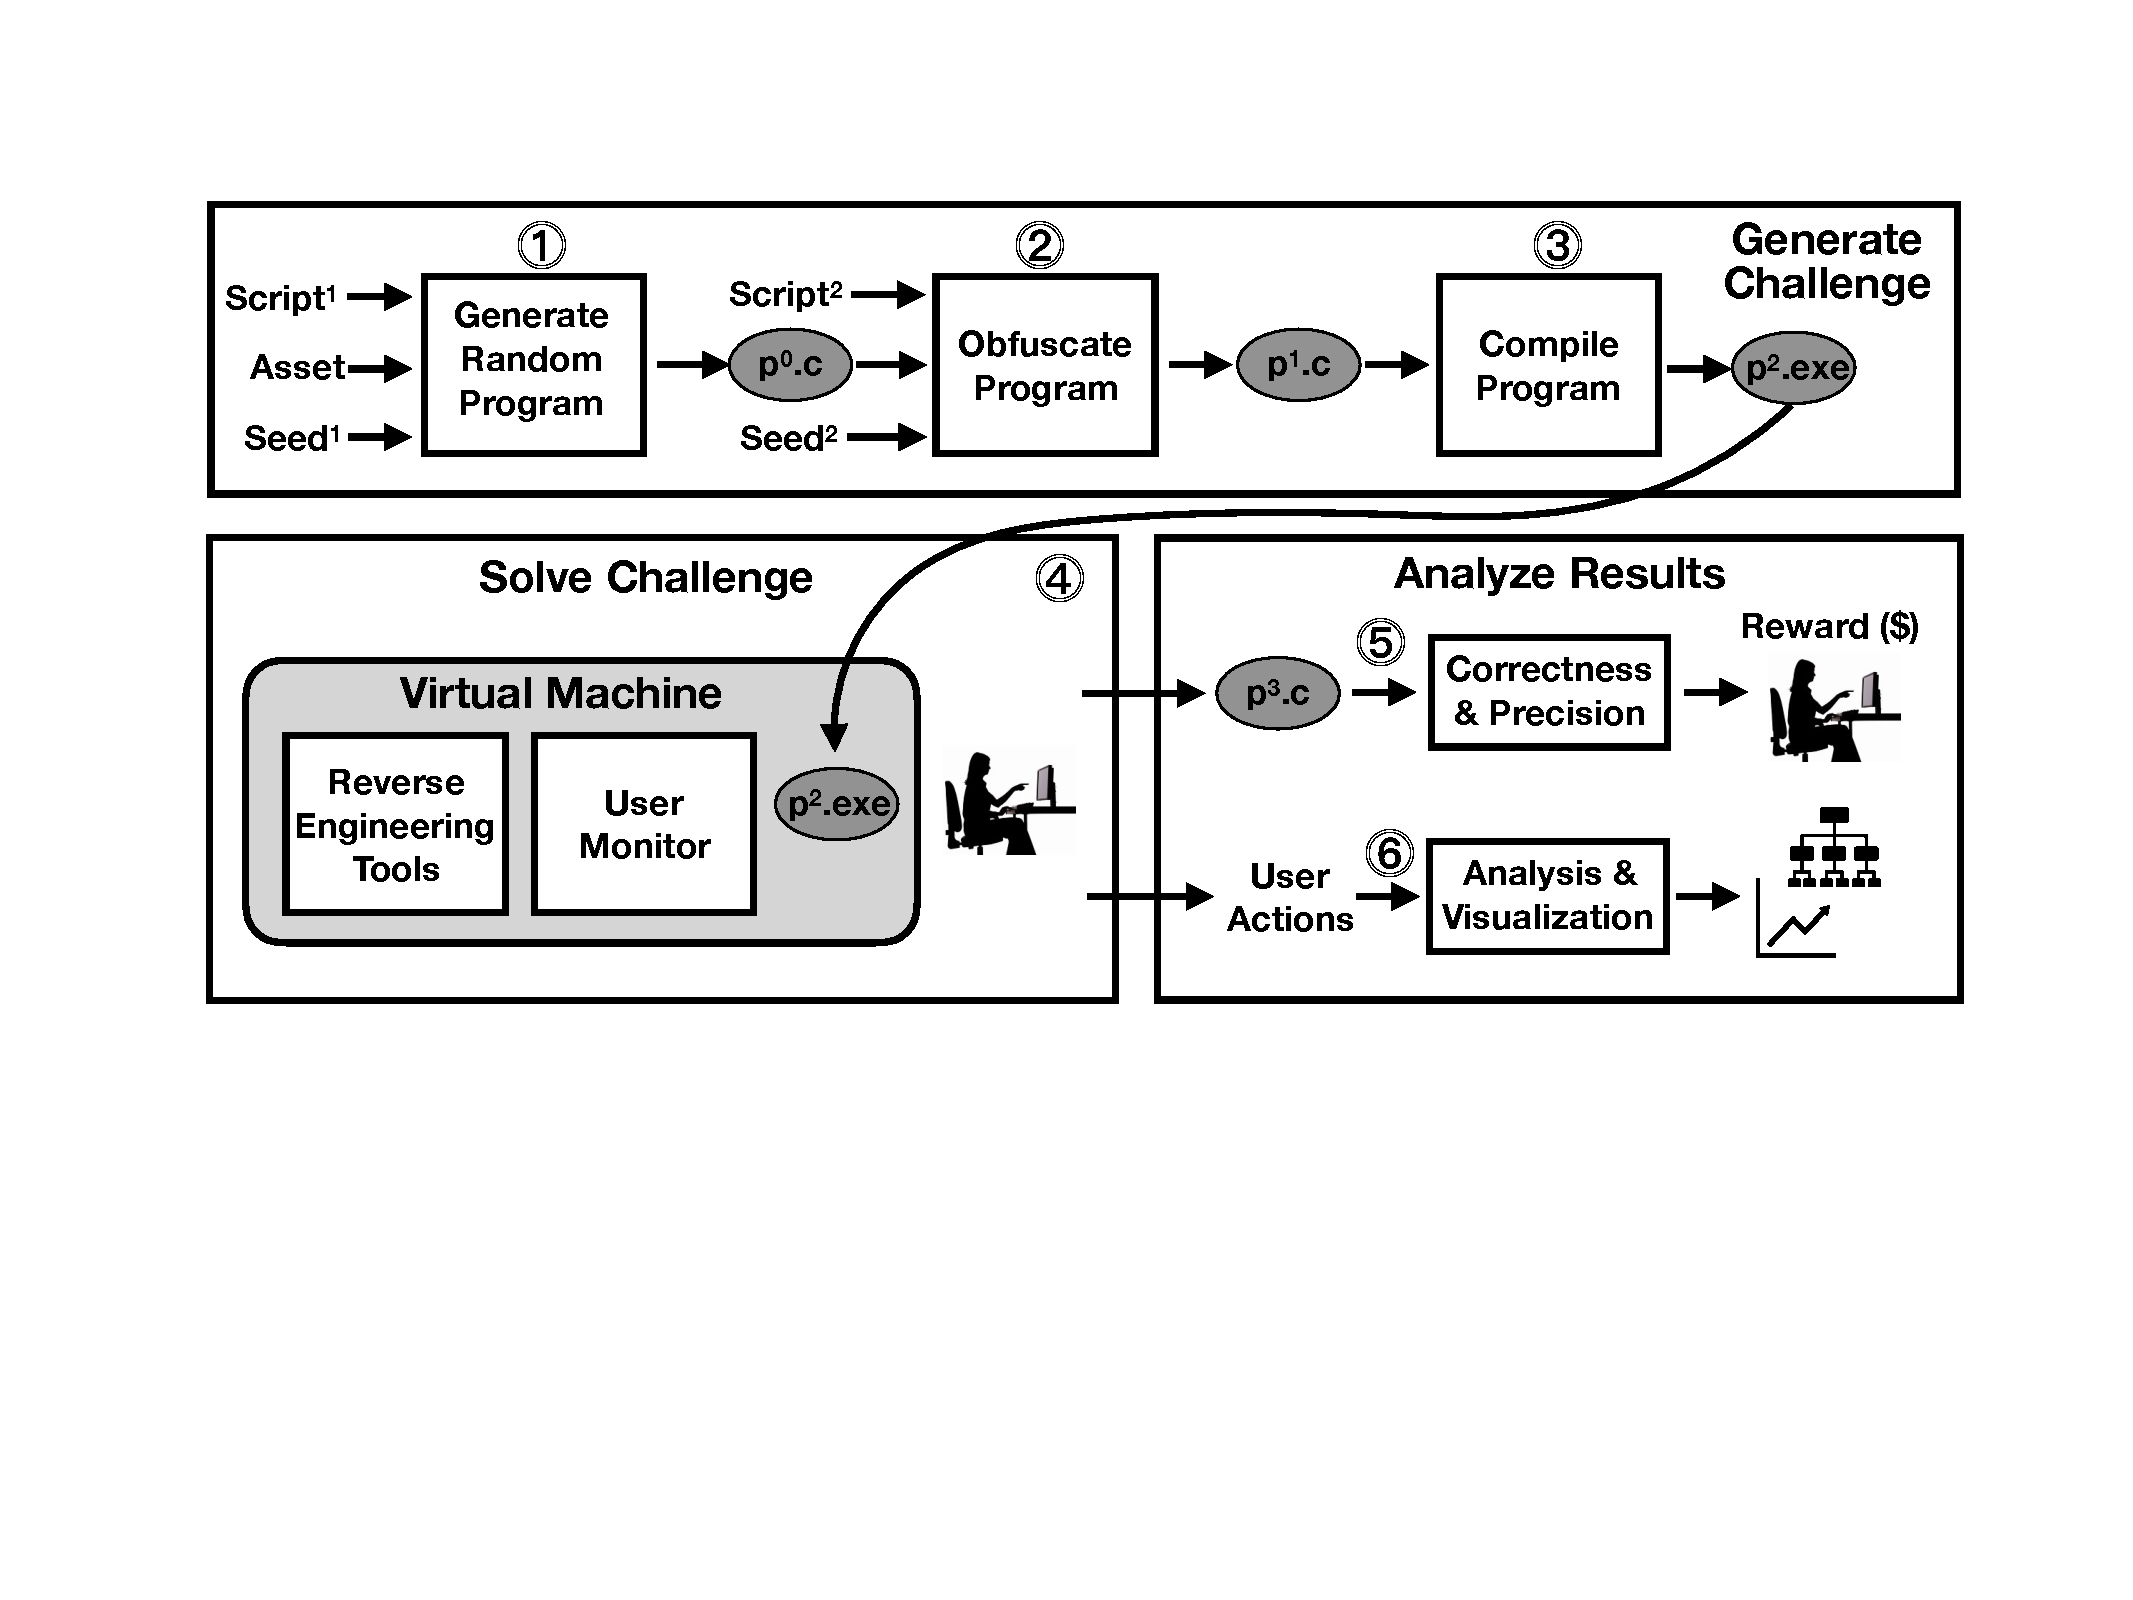
\includegraphics[width=.7\textwidth]{system.pdf}
%\vspace*{-35mm}
%\caption{System Overview.}
%\label{system}
%\end{figure*}

\begin{figure}[t]
\vspace*{-15mm}
\hspace*{-7mm}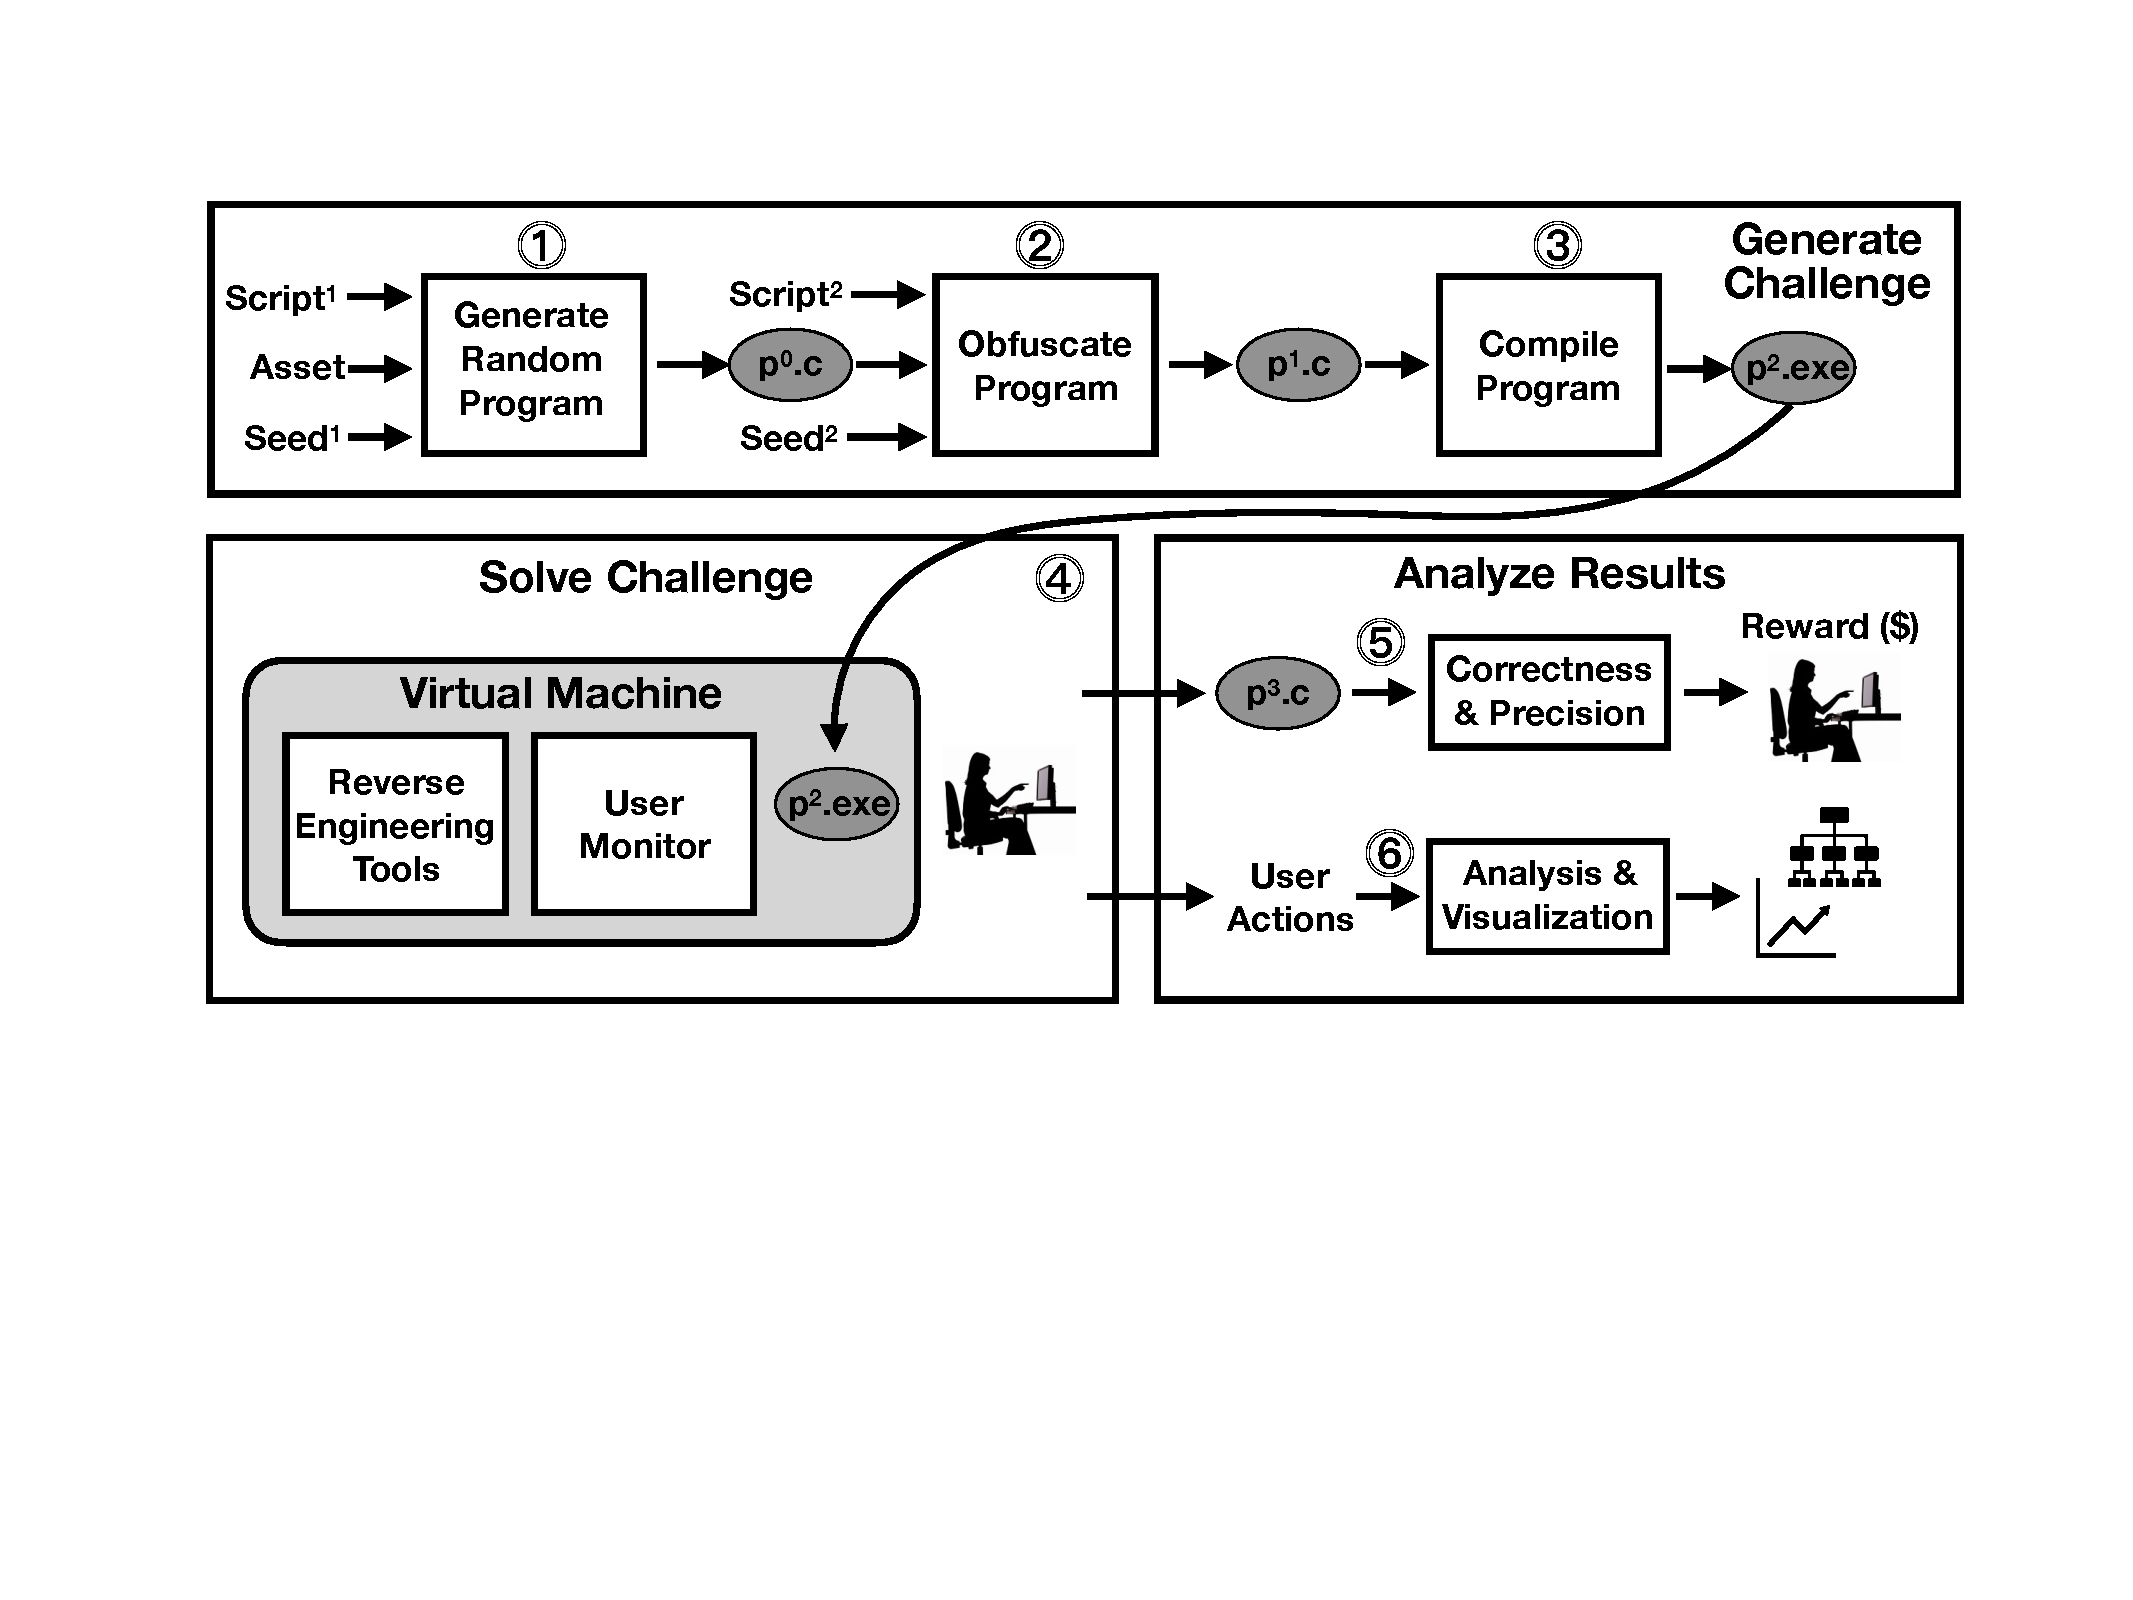
\includegraphics[width=.55\textwidth]{system.pdf}
\vspace*{-30mm}
\caption{System Overview.}
\label{system}
\end{figure}

In the project we report on here, we present a system, \revenge (\revengeExplanation), designed to build models from the behavior of reverse engineers. Figure~\ref{system} shows an overview of the system. Specifically, \revenge generates a secret random program $\mathtt{p}^0.\mathtt{c}$ (point 1 in Figure~\ref{system}) and transforms it with a variety of obfuscating transformations to a program $\mathtt{p}^1.\mathtt{c}$ (point 2) to create a collection of reverse engineering challenges. These challenge programs are made available to reverse engineering experts anywhere to solve (point 3). Experts download the challenge $\mathtt{p}^2.\mathtt{exe}$ into a virtual machine (point 4) equipped with a data collection subsystem that monitors and stores the engineers' behavior as they attempt the challenges. The reverse engineers submit a de-obfuscated solution $\mathtt{p}^3.\mathtt{c}$ which is checked for correctness (point 5). To act as an incentive for accomplished reverse engineers to participate, substantial monetary awards are handed out to successful participants. The recorded user actions are analyzed (point 6) to create reverse engineering attack models, such as visualizations, trees, and Petri nets. The anonymized data set will be made available to the community for further analysis.

This paper is organized as follows.  Section~\ref{relatedwork} discusses related work regarding obfuscation and resilience analysis thereof.  Section~\ref{methodology} presents the design of \revenge. Section~\ref{evaluation} presents an evaluation of the system, and Section~\ref{conclusion} concludes.

%{\em Sharing Statement:} The \revenge system can be accessed at \revengeurl. All the source code is freely available at \sourceurl. The binary for  \tigress used to generate challenges can be downloaded from \tigressurl (source code is available to researchers on request). Properly anonymized data generated by the system will be made freely available to the research community.


